\section{直角坐标系与极坐标系}

坐标系是一种十分基础而重要的数学工具,
它提供了一种简洁的, 确定的方式来描述位置.
\emph{平面直角坐标系}和\emph{极坐标系}
是平面上的两类坐标系, 在弹幕制作中十分常用.

\subsection{平面直角坐标系}

平面直角坐标系在弹幕制作中可以说是最基础的概念之一了,
如果你以前没有见过这个概念,
我说实话还是建议先推进一下三次元世界的学业进度.
之所以还要讲它, 是希望读者能借此熟悉一下本教程的风格.

如图\ref{fig:xy-coord-sys},
平面直角坐标系从直观上像是平面上的一个网格,
有水平和竖直的两条基准线, 称为\emph{坐标轴}.
水平的坐标轴一般称为\emph{横轴}或\emph{$x$轴},
竖直的坐标轴一般称为\emph{纵轴}或\emph{$y$轴}.
两条坐标轴交于一点, 称为\emph{原点}, 一般记作点$O$.
我们可以用$xOy$表示这个坐标系.

在平面直角坐标系中, 每一个点都可以用唯一的有序数对$(x,y)$表示.
对于图\ref{fig:xy-coord-sys}的点$P$,
把$P$分别向$x$轴和$y$轴投影,
在$x$轴上对应的数$x_p = 2$, 称为$P$的\emph{横坐标};
在$y$轴上对应的数$y_p = 1.5$, 称为$P$的\emph{纵坐标};
有序数对$(x_p,y_p) = (2,1.5)$称为$P$的\emph{直角坐标}.

\begin{figure}[htbp]
  \centering
  \begin{tikzpicture}
    \draw[help lines] (-2.2,-1.2) grid (3.2,3.2);
    \draw[-latex] (-2.5,0) -- (3.5,0) node[right]{$x$};
    \draw[-latex] (0,-1.5) -- (0,3.5) node[left]{$y$};

    \foreach \x in {-2,-1,1,2,3} {
        \node[below left] at (\x,0) {\x};
      }
    \foreach \y in {-1,1,2,3} {
        \node[below left] at (0,\y) {\y};
      }

    \draw[dashed] (2,0) |- (0,1.5);
    \draw (0,0) -- (2,1.5);
    \node[dot,label={right:$P$}] at (2,1.5) {};
    \node[dot,label={above right:$A$}] at (2,0) {};
    \node[below left] at (0,0) {$O$};
  \end{tikzpicture}
  \caption{直角坐标系}
  \label{fig:xy-coord-sys}
\end{figure}

在平面直角坐标系中, 我们倾向于在水平和竖直两个方向分别处理问题.
例如, 我们想计算点$A=(x_1,y_1), B=(x_2,y_2)$的中点$C$,
如图\ref{fig:centerpoint},
平面上的一个点可以由一条水平线和一条竖直线确定,
水平线上所有点的纵坐标相等, 竖直线上所有点的横坐标相等.

\begin{figure}[htbp]
  \centering
  \begin{tikzpicture}[declare function={
          x = 2; y = 1;}]
    \foreach \x/\t in {-x/x_1,0/x_c,x/x_2}
    \draw[help lines] (\x,{-(y+0.5)}) -- (\x,{y+0.5})
    node[pos=1,above]{$x=\t$};
    \foreach \y/\t in {-y/y_1,0/y_c,y/y_2}
    \draw[help lines] ({-(x+0.7)},\y) -- ({x+0.7},\y)
    node[pos=0,left]{$y=\t$};

    \draw (-x,-y) -- (x,y);

    \node[dot,label={below right:$C$}] at (0,0) {};
    \node[dot,label={below right:$A$}] at (-x,-y) {};
    \node[dot,label={below right:$B$}] at (x,y) {};
  \end{tikzpicture}
  \caption{中点计算}
  \label{fig:centerpoint}
\end{figure}

我们不难发现 (虽然没有严格证明),
中点$C$的水平线$y = y_c$
应当夹在$A,B$的水平线$y = y_1, y = y_2$之间,
且与这两条水平线的距离相等, 即
\[y_2 - y_c = y_c - y_1,\]
于是$y_c$是$y_1,y_2$的平均数,
即$y_c = \dfrac12 (y_1 + y_2)$.
类似地, 有$x_c = \dfrac12 (x_1 + x_2)$.
所以点$C$的坐标为
\[
  \Big(\dfrac{x_1+x_2}{2},\dfrac{y_1+y_2}{2}\Big).
\]

在解决直角坐标相关的几何问题时, 我们经常会构造直角三角形.
比如要计算图\ref{fig:xy-coord-sys}中$P$与原点$O$的距离,
那么考虑直角三角形$OAP$, 如果已知$P$的直角坐标,
那么线段$OA,AP$的长度是显然的,
而根据$OA,AP$长度就可以求解线段$OP$的长度.
这就引出了\ref{sec:triangle}节对直角三角形边角关系的探讨.
不过这个先放在一边, 我们先看一看另一个常用的坐标系:
极坐标系.

\subsection{任意角}

在我上中学的时候, ``极坐标系''这个概念直到高中才在选修课本中出现,
不过它的内涵在小学时期就已经出现了.
总的来说, 极坐标系通过\emph{距离}和\emph{方位}来确定一个位置.
距离我们知道就是线段长度, 没什么好说的, 那么方位呢?
生活中我们用东南西北四个基本方位结合``偏角''来描述方位,
比如说北偏东30\degree.

在弹幕里我们更希望只用一个数值就能描述一个方位,
在极坐标系中, 这是通过描述\emph{旋转角度}来实现的.
实际上这对应了另一个在高中才出现的概念: \emph{任意角}.

\begin{definition}[任意角]
  如图\ref{fig:angle},
  设平面上有两条射线$AP,AQ$, 它们有共同的起点$A$.
  我们将射线$AP$绕起点$A$旋转到射线$AQ$这个过程称为角,
  记为$\angle PAQ$.
  射线$AP,AQ$分别称为这个角的始边, 终边.
  如果$AP$绕起点$A$逆时针旋转$\alpha$角度
  (或顺时针旋转$-\alpha$) 后到达$AQ$位置,
  那么我们称这个角的大小为$\alpha$.

  \begin{figure}[htbp]
    \centering
    \begin{tikzpicture}[scale=1.2]
      \draw (35:3) -- (0,0) -- (-10:3);
      \node[dot,label={left:$A$}] at (0,0) {};
      \node[dot,label={above:$P$}] at (35:2) {};
      \node[dot,label={below:$Q$}] at (-10:2) {};

      \draw[->] (35:0.5) arc (35:-10:0.5)
      node[right,pos=0.3] {$\alpha = -45\degree$};
      \draw[-latex,help lines] (35:0.5) arc (35:350:0.5)
      node[left,pos=0.45] {$\alpha' = 315\degree$};
    \end{tikzpicture}
    \caption{任意角}
    \label{fig:angle}
  \end{figure}
\end{definition}

任意角的定义和我们最初的角的定义主要有三个方面的区别:
\begin{enumerate}[label=(\arabic*)]
  \item \emph{任意角一定要任意.}
        任意角由旋转操作定义, 而不限制旋转的角度和方向,
        这使得任意角的大小可以是任何数值 (实数),
        包括正数, 零, 负数,
        可以超过360\degree.
  \item \emph{交换始边和终边会改变任意角.}
        传统定义下我们认为$\angle{PAQ}$和$\angle{QAP}$
        表示同一个角, 但对于任意角,
        $\angle{PAQ}$的始边为$AP$, 终边为$AQ$;
        而$\angle{QAP}$的始边为$AQ$, 终边为$AP$.
        二者在某种意义上``互为相反数''.
  \item \emph{即使两个任意角的始边相同, 终边也相同, 它们的值也不一定相等.}
        例如在图\ref{fig:angle}中,
        射线$AP$绕点$A$顺时间旋转45\degree
        或逆时针旋转315\degree 都能得到射线$AQ$,
        所以如果要问图中$\angle{PAQ}$的大小是多少,
        那么答案可以是$-45\degree$ (对应图中$\alpha$),
        也可以是315\degree (对应图中$\alpha'$),
        或其他相差360\degree 的整数倍的值.
\end{enumerate}

任意角以逆时针为正方向, 这是一种人为规定,
LuaSTG在表示速度方向等角度时也使用逆时针正方向.

如果两个任意角相差360\degree 的整数倍,
尽管严格来说这两个角的大小不一定相等,
但它们在大多数应用场景的表现完全相同.
本教程把相差360\degree 的整数倍的两个角$\alpha,\beta$
称为\emph{等价角}, 记作$\alpha\sim\beta$
($\sim$在一些数学领域表示``等价'').
我们会在\ref{sec:modulo}节详细探讨这种关系.

\subsection{极坐标系}

如图\ref{fig:polar-coord-sys},
极坐标系有一个中心点$O$, 称为\emph{极点};
以$O$为起点作一条射线表示0\degree 角, 称为\emph{极轴},
可以沿用直角坐标系的记法, 记为$Ox$;
以逆时针方向为角度的正方向.

对于平面上任一不与极点重合的点$P$,
将极点$O$到点$P$的距离$|OP|$称为点$P$的\emph{极径},
将始边为极轴$Ox$, 终边为$OP$的任意角$\angle{xOP}$称为点$P$的\emph{极角}.
由一个点的极径和极角就可以确定该点的位置.
我们将极径和极角构成的有序数对称为该点的\emph{极坐标},
相对地, 在平面直角坐标系下的坐标称为\emph{直角坐标}.
为了区分直角坐标和极坐标的表示,
本教程用\emph{尖括号$\braket{}$}表示极坐标.
例如图\ref{fig:polar-coord-sys}的点$P$,
它的极径$r_p = 2.5$, 极角$\theta_p = 45\degree$,
极坐标为 $\braket{r_p,\theta_p} = \braket{2.5,45\degree}$.

\begin{figure}[htbp]
  \centering
  \begin{tikzpicture}[scale=0.7]
    \foreach \a in {0,30,...,330}
    \draw[help lines] (0,0) -- (\a:3.2);
    \foreach \r in {1,2,3}
    \draw[help lines] (0,0) circle (\r);

    \coordinate (P) at (45:2.5);

    \draw[] (0,0) node[dot] {}
    -- (P) node[dot,label={[background]right:$P$}] {};
    \draw[-latex] (0,0) -- (3.5,0)
    node[right]{$0\degree$};

    \begin{scope}[below]
      \node[background] at (0,0) {$O$};
      \foreach \x in {1,2,3}
      \node[background] at (\x,0) {\x};
    \end{scope}

    \foreach \a in {90,180,270}
    \node[anchor={\a+180}] at (\a:3.2) {$\a\degree$};
    \foreach \a in {30,60,120,150,210,240,300,330}
    \node[anchor={\a+180},help lines] at (\a:3.2) {$\a\degree$};
  \end{tikzpicture}
  \caption{极坐标系}
  \label{fig:polar-coord-sys}
\end{figure}

特别规定, 极点$O$的极坐标为$\braket{0,\theta}$,
其中$\theta$可以为任意数值.

由于任意角的性质, 一个位置对应无穷多个极坐标
(相对地, 一个位置对应恰好一个直角坐标).
例如, 将图\ref{fig:polar-coord-sys}的点$P$绕极点旋转360\degree,
点$P$的位置不变, 所以$\braket{r,\theta}$
和$\braket{r,\theta+360\degree}$表示同一个位置.
类似地, $\braket{-r,\theta}$和
$\braket{r,\theta+180\degree}$也表示同一个位置.

为了缓解这个问题, 我们可以对极径和极角的取值加以限制.
通常我们规定极径不小于0 (两点的距离不会是负数, 对吧),
这样一个位置的极径就是唯一的了.
尽管极角仍然不唯一, 但一个位置所有可能的极角都是等价的,
代表相同的方向, 基本没什么问题.
至于极点, 它的极角本来就是未定义的, 没有实际意义.
另外, 如果我们额外限制$-180\degree < 极角 \le 180\degree$,
或者$0\degree \le 极角 < 360\degree$之类的,
那么非极点的每个点都能对应唯一的极坐标.

\subsection*{碎碎念}

在弹幕制作中我们经常用速度大小和方向描述速度 (以及加速度),
这其实就是极坐标系的一个应用, 虽然这时并没有涉及极坐标系这个名词.
速度大小就是极径, 速度方向就是极角.
到这里至少我是有一种感觉,
我们似乎根本不需要去额外用一套``极坐标''的术语
来表达我们已经非常熟悉的``用大小和方向来表达位置''的体系,
``黑话''太多只会徒增记忆和交流难度而已\cndots

一方面, ``极坐标''这套术语提供了一种方法来表达
用距离和方位确定位置的一种\emph{坐标系}, 在数学上并非冗余,
而弹设们引用这套术语, 主要是因为极坐标方程
\footnote{
  如果你接触过形如$x^2+y^2=1$的曲线方程的话,
  极坐标方程就是关于极径和极角的方程,
  被用来描述一些比较特殊的曲线
},
也是因为有需求才引入的术语.

但另一方面, 像``极坐标'' ``向量'' ``矩阵''
这类比较``拉风''的术语有时会作为某种``行业黑话''被滥用.
比如有新手在群里问一个东西怎么实现,
就可能会出现一些人直接把这些术语甩出来而不做额外解释,
然后新手就只能上网瞎找然后直呼看不懂,
最后也不知是福是祸了
\footnote{不知福祸? 那就是\underline{\makebox[6mm]{}}}.
当然他们这样做是有一些理由的,
比如没时间细讲, 懒, 或者觉得新人知道术语自己学学就够了,
或者有一些东西确实是不太好讲, 等等.

虽然我不能真的要求什么, 但我还是希望群友在解答新人问题时,
要么不发言, 要发言, 就照顾一下新人的情况,
少用点术语, 多讲点人话. 新人提问没人解答冷场事小,
得了敷衍的解答, 反复受折腾遭的罪可大啊\cndots

我写下这个教程, 也是希望看到这个教程的人能了解到,
我们使用的那些看似是高中甚至大学才会学到的数学术语,
它们要表达的内容其实是足够浅显的;
我们或许做得一手好弹幕却对这些术语完全没有了解,
但是术语背后蕴含的内容以及思维方式, 我们是一直在运用的.

\subsection*{习题}

\begin{enumerate}
  \item \comment{坐标系转换v1}
        我们在描述子弹的坐标时使用一个
        以版面中心为原点, 以右上为正方向的直角坐标系,
        即图\ref{fig:board-v1}所示的$xOy$坐标系,
        这个坐标系在LuaSTG中称为\raw{world}坐标系.
        而在处理游戏UI相关的渲染, 例如, 界面右侧的残机数等数据显示时,
        我们需要切换到\raw{ui} view mode进行处理,
        而这个view mode使用另一个坐标系,
        即图\ref{fig:board-v1}中的$x'O'y'$坐标系.
        需要在这个坐标系下确定渲染的位置.

        总之, 这道题目探讨\raw{world}坐标系$xOy$和
        \raw{ui}坐标系$x'O'y'$的坐标转换.
        假设我们要在\raw{ui}坐标系渲染版底的
        boss指示标记 (在图中用点$P$表示).
        我们容易知道它在\raw{world}坐标系的坐标:
        横坐标与boss保持一致 (但是不超出版面),
        纵坐标为版底 ($-224$).

        正常我们需要处理LuaSTG内置的一堆参数,
        但这是第一道习题所以我们简化一下.
        那么题目是这样的:

        如图\ref{fig:board-v1}, 设平面上有$xOy,x'O'y'$
        两个平面直角坐标系, 它们的$x$轴和$y$轴的
        正方向相同, 单位长度
        \footnote{单位长度就是, ``1''代表多大的长度.}
        也相同, 但是原点$O,O'$的位置不同.
        已知在$x'O'y'$坐标系中, 点$O$的坐标为$(224,240)$,
        而在$xOy$坐标系中, 点$P$的坐标为$(x_p,y_p)$,
        求点$P$在$x'O'y'$坐标系下的坐标.

        \begin{figure}[htbp]
          \centering
          \begin{tikzpicture}
            \node[
              anchor=south west,
              inner sep=0pt,
              outer sep=0pt
            ] (image) at (0,0)
            {\includegraphics[width=10cm]{assets/coord/board-v1.png}};

            \begin{scope}[
                x={(image.south east)},
                y={(image.north west)},
              ]
              \coordinate (O) at (224/640,240/480);
              \coordinate (Oxx) at (1,240/480);
              \coordinate (Ox) at (1.1,240/480);
              \coordinate (Oyy) at (224/640,1);
              \coordinate (Oy) at (224/640,1.1);

              \draw[latex-latex,very thick]
              (1.1,0) -- (0,0) -- (0,1.1);
              \draw[white,very thick]
              (Oxx) -- (O) -- (Oyy);
              \draw[-latex,very thick] (Oxx) -- (Ox);
              \draw[-latex,very thick] (Oyy) -- (Oy);


              \node[dot,label={left:$O'$}] at (0,0) {};
              \node[right] at (1.1,0) {$x'$};
              \node[left] at (0,1.1) {$y'$};
              \node[white,dot,label={[white]left:$O$}] at (O) {};
              \node[right] at (Ox) {$x$};
              \node[left] at (Oy) {$y$};

              \node[dot,white,label={[white]left:$P$}]
              at ({224/640},{(240-224)/480}) {};
            \end{scope}
          \end{tikzpicture}
          \caption{LuaSTG版面}
          \label{fig:board-v1}
        \end{figure}

  \item \comment{镜面反射v1*}
        反弹子弹是一种比较常见的运动模式,
        一个典型的例子是符卡QED\spellcard{495年的波纹},
        你可以在DEMO2弹幕工程中看到反弹的实现方式.
        考虑一个比较简单的反弹:
        一个子弹做匀速直线运动, 它的贴图方向和运动方向相同,
        当某一帧我们检测到子弹离开版面时,
        我们需要改变它的朝向 (贴图朝向和速度方向).

        \begin{figure}[htbp]
          \centering
          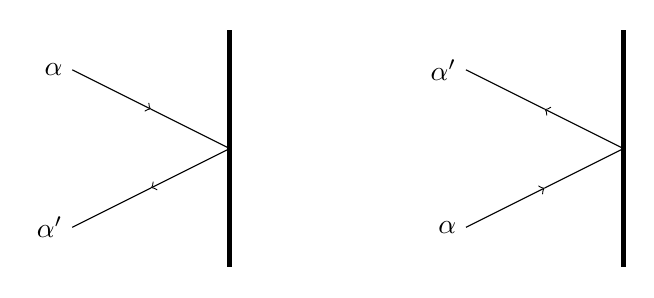
\begin{tikzpicture}
            \draw[line width=2pt] (0,-1.5) -- (0,1.5);
            \draw[->] (-2,1) -- (-1,0.5);
            \draw[->] (-1,0.5) -- (0,0) -- (-1,-0.5);
            \draw (-1,-0.5) -- (-2,-1);
            \node[left] at (-2,1) {$\alpha$};
            \node[left] at (-2,-1) {$\alpha'$};

            \begin{scope}[xshift=5cm]
              \draw[line width=2pt] (0,-1.5) -- (0,1.5);
              \draw (-2,1) -- (-1,0.5);
              \draw[<-] (-1,0.5) -- (0,0) -- (-1,-0.5);
              \draw[<-] (-1,-0.5) -- (-2,-1);
              \node[left] at (-2,1) {$\alpha'$};
              \node[left] at (-2,-1) {$\alpha$};
            \end{scope}
          \end{tikzpicture}
          \caption{反弹/镜面反射}
          \label{fig:rebound-v1}
        \end{figure}

        \begin{enumerate}[label=(\alph*)]
          \item 考虑子弹在版面右侧的反弹, 如图\ref{fig:rebound-v1},
                检测到子弹到达版面右侧时, 子弹的朝向为$\alpha$角,
                请计算反弹后子弹的朝向$\alpha'$角
                (一个可能取值即可).
                子弹原来的朝向$\alpha$会改变$\alpha'$的计算结果吗?
        \end{enumerate}

        小明让一圈简单子弹围成圆形, 开启rebound来实现反弹.
        但是他发现, 子弹在反弹后不再围成圆形,
        而是形成一个奇怪的形状,
        如图\ref{fig:rebound-v1-error}. 出现这种错误,
        是因为LuaSTG简单子弹的反弹在实现上有一点缺陷,
        没有考虑到反弹时子弹坐标应该发生改变
        (不知道什么时候会修复).

        \begin{figure}[htbp]
          \centering
          \includegraphics[width=10cm]{assets/coord/rebound-error.png}
          \caption{出错的反弹}
          \label{fig:rebound-v1-error}
        \end{figure}

        具体来说, 游戏是一帧帧运行的, 在某一帧我们检测到子弹离开版面时,
        它几乎不会恰好在边界上, 而是总与边界有一段距离.
        如图\ref{fig:rebound-v1-points},
        假设我们检测到需要反弹时, 子弹位于点$P$.
        在左侧的例子中, 我们只改变子弹的朝向,
        可以看到子弹反弹后的运动轨迹与我们想要的反弹轨迹有一定的偏差;
        更糟糕的是, 由于不同子弹离开版面时与边界的距离不同,
        它们反弹后的轨迹无法对齐, 也就导致原来构成圆形的一群子弹
        在反弹后形状受到破坏.

        \begin{figure}[htbp]
          \centering
          \begin{tikzpicture}
            \draw[line width=2pt] (0,-1.5) -- (0,1.5);
            \begin{scope}[shift=(150:-0.7)]
              \draw[help lines] (150:3.5) -- (0,0) -- (-150:2.5);
              \foreach \r in {0,1,2,3}
              \node[dot] at (150:\r) {};
              \foreach \r in {1,2}
              \node[dot] at (-150:\r) {};
              \node[right] at (0,0) {$P$};
            \end{scope}
            \draw[->] (-2.5,1) -- +(-30:0.4);


            \begin{scope}[xshift=7cm]
              \draw[line width=2pt] (0,-1.5) -- (0,1.5);
              \draw[help lines] (150:3) -- (0,0) -- (-150:3);
              \draw[help lines,dashed] (0,0) -- (-30:1.5);
              \foreach \r in {2.3,1.3,0.3,-0.7}
              \node[dot] at (150:\r) {};
              \foreach \r in {0.7,1.7}
              \node[dot] at (-150:\r) {};
              \draw[->] (-2.5,1) -- +(-30:0.4);
              \draw[dashed]
              (-30:0.7) node[right] {$P$}
              -- (30:-0.7) node[left] {$P'$};
            \end{scope}
          \end{tikzpicture}
          \caption{错误与正确的反弹}
          \label{fig:rebound-v1-points}
        \end{figure}

        为了修复这个错误, 我们需要在反弹时改变子弹的坐标.
        在图中右侧的例子中, $P'$是在正确的反弹轨迹上点$P$的对应位置.
        我们可以发现, $P,P'$实际上是轴对称的 (相对于反弹边界).

        \begin{enumerate}[label=(\alph*),start=2]
          \item 设检测到子弹离开版面时,
                子弹的坐标为$P = (x_p,y_p)$,
                对应的反弹边界是右边界$x = 192$,
                点$P'$是点$P$关于该反弹边界的轴对称点.
                求$P'$的坐标.
        \end{enumerate}
\end{enumerate}
